% !TeX program = pdflatex
\documentclass[12pt,a4paper,oneside]{extarticle}
%\usepackage{xunicode} % https://ctan.org/pkg/xunicode
%\usepackage{xltxtra} % https://ctan.org/pkg/xltxtra
\usepackage{fontspec} % https://ctan.org/pkg/fontspec
\usepackage{polyglossia} % https://ctan.org/pkg/polyglossia
\setdefaultlanguage{portuges}
%\setdefaultlanguage{portuguese}
%\setdefaultlanguage[spelling=old]{portuguese}
\usepackage{csquotes}

%\usepackage{ebgaramond}%[RawFeature={+onum,+pnum,+ss06}]
\usepackage[cmintegrals,cmbraces]{newtxmath}
%\usepackage{ebgaramond-maths}

\usepackage[no-math]{fontspec}
%\setmainfont{EBGaramond}[
%  Extension=.otf,
%  UprightFont=*-Regular,
%  ItalicFont=*-Italic,
%  BoldFont=*-Bold,
%  BoldItalicFont=*-BoldItalic,
%  Numbers={Proportional,OldStyle},
%  Ligatures=TeX
%]

%\setmainfont{TeX Gyre Pagella}[
%  Extension = .otf,
%  UprightFont = *-Regular,
%  ItalicFont = *-Italic,
%  BoldFont = *-Bold,
%  BoldItalicFont = *-BoldItalic,
%  Ligatures = TeX
%]



\clubpenalty=100
\linepenalty=100
\widowpenalty=100

%estética
% \usepackage[hyphens]{url}
\usepackage{xurl}
\urlstyle{same} % URLs na mesma fonte do texto (Times New Roman)
\AtBeginDocument{%
  \setlength{\Urlmuskip}{0mu plus 1mu} % Ajusta espaçamento entre caracteres em URLs
  \setlength{\emergencystretch}{3em} % Permite maior flexibilidade na justificação
  \def\UrlBreakPenalty{100} % Penalidade baixa para facilitar quebras
  \def\UrlBigBreakPenalty{50} % Penalidade para quebras em caracteres como /
  \sloppy % Relaxa a justificação para evitar ultrapassagem
}

\usepackage[hang,small,bf]{caption}
\usepackage[a4paper,left=2.5cm,right=2.5cm,top=2.5cm,bottom=2.5cm,includehead,includefoot]{geometry}
\linespread{1.3}

\usepackage[
  xetex,                      % Driver para XeLaTeX
  unicode=true,               % Suporte a caracteres Unicode (ex.: ç, ã)
  bookmarks=true,             % Cria bookmarks no PDF
  bookmarksopen=true,         % Bookmarks abertos por padrão
  bookmarksnumbered=true,     % Numera os bookmarks (ex.: 1, 1.1, 1.2)
  linktoc=all,                % Links clicáveis em sumário, figuras e citações
  breaklinks=true,            % Permite quebra de links longos
  colorlinks=true,            % Links com cor em vez de caixas
  citecolor=black,            % Cor das citações (preto)
  filecolor=black,            % Cor dos links de arquivos (preto)
  linkcolor=black,            % Cor dos links internos (preto)
  urlcolor=blue,              % URLs em azul
  pdfpagelabels=true,         % Adiciona rótulos às páginas do PDF
  plainpages=false,           % Diferencia numeração de páginas
  pdftitle={Desafios 12 ano},
  pdfauthor={Desafios 12 ano}, % Nome do autor
  pdfsubject={Desafios 12 ano},
  pdfkeywords={Desafios 12 ano},
  pdfcreator={XeLaTeX com hyperref},
  pdfproducer={XeLaTeX}
]{hyperref}

%% Definir um novo estilo de url
\makeatletter
\def\url@luisstyle{%
  \@ifundefined{selectfont}{\def\UrlFont{\sf}}{\def\UrlFont{\small\ttfamily}}}
\makeatother
\urlstyle{luis}

\setlength{\captionmargin}{1.5in}
\usepackage{fancyhdr}

\renewcommand{\thefootnote}{\alph{footnote}} %modificar as letras de notas de rodapé%
\makeatletter
\renewcommand\@makefnmark{\@textsuperscript{\normalfont(\@thefnmark)}}
\makeatother
\renewcommand{\fboxrule}{2pt} %para alterar a expessura das caixas
%\renewcommand{\fboxsep}{3ex} %para alterar a separação nas caixas

%para alterar a fonte dos items http://cnlart.web.cern.ch/cnlart/214/node68.html
%\renewcommand{\labelenumi}{\textbf{\arabic{enumi}.}}
\renewcommand{\labelenumi}{\textbf{\alph{enumi}.}}
%\renewcommand{\labelenumii}{\textbf{\alph{enumii}.}}
%\renewcommand{\labelenumii}{\textbf{(\alph{enumii})}}
\renewcommand{\labelenumii}{\textbf{(\arabic{enumii})}}

\long\def\symbolfootnote[#1]#2{\begingroup\def\thefootnote{\fnsymbol{footnote}}\footnote[#1]{#2}\endgroup}

%%%%%%%%%%%%%%%%%%%%%%%%%%%%
%%%%%%%%%%%%%%%%%%%%%%%%%%%%
%%%%%%%%%%%%%%%%%%%%%%%%%%%%
\usepackage{setspace}
%\singlespacing
%\onehalfspacing
%\doublespacing

\usepackage{comment}
\usepackage{siunitx}
%%%%%%%%%%%%%%%%%%%%%%%%%%%%
\usepackage[x11names]{xcolor} 
%%%%%%%%%%%%%%%%%%%%%%%%%%%%
\usepackage{relsize}
%\newcommand\CC{C\nolinebreak\hspace{-.05em}\raisebox{.4ex}{\relsize{-3}{\textbf{+}}}\nolinebreak\hspace{-.10em}\raisebox{.4ex}{\relsize{-3}{\textbf{+}}}}
\newcommand\CC{C\nolinebreak[4]\hspace{-.05em}\raisebox{.4ex}{\relsize{-3}{\textbf{++}}}}

%\usepackage{showframe}
\usepackage{pgf,tikz}       % - Elementos gráficos
\usepackage{tikzpagenodes}
\usetikzlibrary{backgrounds,calc,positioning}
\usetikzlibrary{positioning, shapes}

\pgfdeclarelayer{background}
\pgfdeclarelayer{foreground}
\pgfsetlayers{background,main,foreground}

\usepackage[
    backend=biber,
    style=numeric-comp,
    language=auto,
    natbib=false,
    block=space,
    isbn=false,
    url=true, 
    doi=true,
    mcite=true,
    eprint=false,
    sorting=none,
    maxnames=6
]{biblatex} % https://ctan.org/pkg/biblatex
\addbibresource{bibliografia.bib}


\begin{document}
%espaço negativo para o cabeçalho
\vspace*{-2cm}
\begin{tikzpicture}[remember picture, overlay]
  \draw[line width = 0.5pt, color=black] ($(current page.north west) + (2.5cm,-2cm)$) -- ($(current page.north east) + (-2.5cm,-2cm)$);
\end{tikzpicture}
\vspace*{2mm}
\begin{minipage}[c][2.5cm][t]{.25\textwidth}
    
\includegraphics[width=\linewidth]{logos/aeB06.pdf}
\end{minipage}\hfill
\begin{minipage}[c][2.5cm][t]{.7\textwidth}
	\begin{center}\Large\textbf{Agrupamento de Escolas de Benfica}\end{center}
	\vspace{-8.5mm}
	\begin{center}\large\textbf{Escola Secundária José Gomes Ferreira}\end{center}
	\vspace{-8.5mm}
	\begin{center}\large{Grupo Disciplinar 510}\end{center}
\end{minipage}
\begin{tikzpicture}[remember picture, overlay]
\draw[line width = 0.5pt, color=black] ($(current page.north west) + (2.5cm,-4.8cm)$) -- ($(current page.north east) + (-2.5cm,-4.8cm)$);
\end{tikzpicture}
\vspace{10mm}
\begin{center}
\Large{\textbf{Análise e Implementação Computacional da Geometria dos Favos de Mel}}\par 
\large{\textbf{Adrian Dias}}\par 
\large{\textbf{Nº 1, T 12º 3ª }}\par 
\Large{-- Disciplina de Física --}\par
\textbf{2025 - 2026}\\
\end{center}

\begin{tikzpicture}[remember picture, overlay]
  \draw[line width = 0.5pt, color=black] ($(current page.south west) + (2.5cm,3cm)$) -- ($(current page.south east) + (-2.5cm,3cm)$);
\end{tikzpicture}


\begin{abstract}
Este relatório apresenta o desenvolvimento de um modelo matemático e a respectiva implementação em \texttt{Python}/\texttt{turtle}, com vista à representação de uma concha do náutilus encontrada na natureza. São descritos os objectivos, a metodologia seguida e os principais resultados obtidos. 
\end{abstract}

\section{Introdução}
Neste capítulo apresenta-se o enquadramento teórico do trabalho, incluindo o modelo matemático de base e o modelo específico implementado no código.

\subsection{Modelo Matemático da Espiral Logarítmica (1.1)}
A concha do náutilus segue uma espiral logarítmica, também conhecida como espiral de crescimento ou espiral equiangular. Esta curva é representada pela equação polar:

\begin{equation}
r(\theta) = a \cdot e^{b \cdot \theta}
\label{eq:espiral}
\end{equation}

\noindent onde:
\begin{itemize}
    \item $r$ é o raio da espiral (distância do ponto à origem)
    \item $\theta$ é o ângulo em radianos (parâmetro angular)
    \item $a$ é o raio inicial (constante de escala que determina o tamanho inicial)
    \item $b$ é a taxa de crescimento (controla a "abertura" ou "fechamento" da espiral)
    \item $e$ é a base do logaritmo natural ($e \approx 2.71828$)
\end{itemize}

\subsection{Propriedades Matemáticas Fundamentais (1.2)}
A espiral logarítmica possui propriedades matemáticas notáveis que explicam sua prevalência na natureza:

\begin{itemize}
    \item \textbf{Auto-similaridade}: A forma mantém-se invariante sob transformações de escala. Isto significa que qualquer secção da espiral é geometricamente similar à espiral completa.
    
    \item \textbf{Ângulo constante}: O ângulo $\alpha$ entre o raio vetor e a tangente à curva é constante em todos os pontos, satisfazendo a relação $\cot(\alpha) = b$.
    
    \item \textbf{Crescimento exponencial}: O raio cresce exponencialmente com o ângulo, o que corresponde a uma taxa de crescimento proporcional ao tamanho atual.
    
    \item \textbf{Propriedade de crescimento isomórfico}: A forma da espiral mantém-se constante durante o crescimento, o que é energeticamente eficiente para organismos vivos.
\end{itemize}

\subsection{Implementação Computacional (1.3)}
No script \texttt{Python/turtle}, a equação~\ref{eq:espiral} é implementada através da conversão de coordenadas polares para cartesianas:

\begin{equation}
x = r(\theta) \cdot \cos(\theta), \quad y = r(\theta) \cdot \sin(\theta)
\label{eq:cartesianas}
\end{equation}

Para criar a forma tridimensional da concha, utilizou-se o conceito de faixa espiral, onde uma segunda espiral com raio $r_2(\theta) = r_1(\theta) + d(\theta)$ é desenhada, sendo $d(\theta)$ uma função que define a largura da concha.

\subsection{Formulação por Equações Diferenciais (1.4)}
A espiral logarítmica surge naturalmente de sistemas dinâmicos. Considerando o sistema:

\begin{equation}
\begin{cases}
\dot{x} - \dot{y} = \ddot{x}\sqrt{\dot{x}^2 + \dot{y}^2} \\
\dot{x} + \dot{y} = \ddot{y}\sqrt{\dot{x}^2 + \dot{y}^2}
\end{cases}
\label{eq:diferencial}
\end{equation}

A solução em coordenadas polares conduz ao sistema:

\begin{equation}
\dot{r} = 1, \quad \dot{\theta} = \frac{1}{r}
\end{equation}

cuja solução é a espiral logarítmica $r = c_0 \cdot e^\theta$, demonstrando como padrões naturais emergem de leis dinâmicas simples.

\subsection{Propriedade de Inversão (1.5)}
A inversão da espiral logarítmica no círculo unitário, dada por $r_{inv}(\theta) = 1/r(\theta)$, produz outra espiral logarítmica. Esta propriedade é particularmente relevante em transformações geométricas e mapeamentos conformes.

\subsection{Cálculo de Áreas na Concha (1.6)}
A área de uma secção da concha pode ser calculada através da integral:

\begin{equation}
A = \frac{1}{2}\int_{\theta_1}^{\theta_2} r^2 d\theta = \frac{1}{2}\int_{\theta_1}^{\theta_2} a^2 e^{2b\theta} d\theta = \frac{a^2}{4b}(e^{2b\theta_2} - e^{2b\theta_1})
\label{eq:area}
\end{equation}

Para a concha do náutilus, consideramos normalmente $\theta_1 = 6\pi$ e $\theta_2 = 8\pi$ para a última revolução, resultando numa área que cresce exponencialmente com cada volta.

\subsection{Modelo de Faixa Espiral para Conchas (1.7)}
Para representar a concha 3D, utilizou-se o modelo de faixa espiral com duas espirais concêntricas:

\begin{equation}
\begin{cases}
r_1(\theta) = a \cdot e^{b\theta} & \text{(espiral interna)} \\
r_2(\theta) = r_1(\theta) + d(\theta) & \text{(espiral externa)}
\end{cases}
\label{eq:faixa}
\end{equation}

onde $d(\theta)$ representa a largura da concha. A área da secção transversal da última revolução é dada por:

\begin{equation}
A_{seccao} = \frac{1}{2}\int_{6\pi}^{8\pi} [r_2^2(\theta) - r_1^2(\theta)] d\theta
\label{eq:area_seccao}
\end{equation}

No caso de uma concha real, $d(\theta)$ tipicamente aumenta com $\theta$ para acomodar o crescimento do organismo.

\subsection{Parâmetros e Ajuste}
Os parâmetros $a$ e $b$ foram ajustados empiricamente para aproximar a forma de uma concha real:
\begin{itemize}
    \item $a = 2.0$: Define o tamanho inicial da concha
    \item $b = 0.22$: Controla a taxa de abertura da espiral
    \item $\theta \in [0, 8\pi]$: Permite 4 voltas completas da espiral
    \item $d(\theta) = 0.4 \cdot r(\theta)$: Largura proporcional ao raio atual
\end{itemize}

\begin{figure}[ht!]
    \centering
    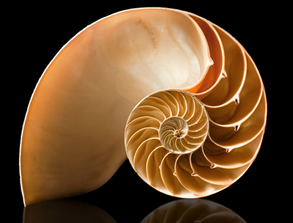
\includegraphics[width=0.6\textwidth]{figuras/nautilus.png}
    \caption{Concha do Náutilus - modelo matemático implementado em Python/turtle.}
    \label{fig:referencia}
\end{figure}
  
\section{Parte Experimental}
A componente experimental deste trabalho corresponde à elaboração e explicação do código em \texttt{Python} com a biblioteca \texttt{turtle}. Tal como num procedimento laboratorial, importa detalhar a lógica implementada, os algoritmos utilizados e as opções tomadas em cada etapa, de forma a permitir a replicação do processo.

\subsection{Arquitetura do Código}
O script foi estruturado em funções modulares para facilitar a compreensão e manutenção:

\begin{itemize}
    \item \texttt{espiral\_logaritmica(a, b, theta)}: Calcula pontos na espiral
    \item \texttt{desenhar\_concha\_realista()}: Função principal de desenho
    \item \texttt{desenhar\_camaras(pontos)}: Adiciona divisórias internas
    \item \texttt{desenhar\_estrias()}: Cria linhas de crescimento
\end{itemize}

\subsection{Implementação da Espiral Logarítmica}
A equação fundamental $r(\theta) = a \cdot e^{b\theta}$ foi implementada da seguinte forma:

\begin{verbatim}
def espiral_logaritmica(a, b, theta):
    r = a * math.exp(b * theta)
    x = r * math.cos(theta)
    y = r * math.sin(theta)
    return x, y, r
\end{verbatim}

\subsection{Conversão Coordenadas Polares-Cartesianas}
Para compatibilidade com o sistema \texttt{turtle}, as coordenadas polares são convertidas:

\begin{equation}
x = r \cdot \cos(\theta), \quad y = r \cdot \sin(\theta)
\end{equation}

O incremento angular $\Delta\theta = 0.01$ radianos garante suavidade na curva.

\subsection{Modelo de Faixa Espiral}
Para criar a espessura da concha, implementou-se o conceito de faixa espiral com duas curvas:

\begin{verbatim}
# Espiral interna
r1 = a * math.exp(b * theta)
# Espiral externa  
r2 = r1 + 0.4 * r1  # Largura proporcional
\end{verbatim}

\subsection{Parâmetros Ajustados}
Através de testes iterativos, determinou-se os parâmetros ótimos:

\begin{itemize}
    \item \textbf{a = 2.0}: Tamanho inicial que equilibra visualização e detalhe
    \item \textbf{b = 0.22}: Taxa de crescimento que produz forma realista
    \item \textbf{Ângulo total}: $8\pi$ radianos (4 voltas completas)
    \item \textbf{Resolução}: 800 pontos para suavidade adequada
\end{itemize}

\subsection{Algoritmo de Desenho}
O desenho segue a sequência:

\begin{enumerate}
    \item Inicialização do ambiente \texttt{turtle}
    \item Desenho da espiral interna (do centro para fora)
    \item Desenho da espiral externa (retorno)
    \item Preenchimento da área entre espirais
    \item Adição de elementos detalhados (câmaras, estrias)
\end{enumerate}

\subsection{Otimizações Implementadas}
Para melhor performance e qualidade visual:

\begin{itemize}
    \item \textbf{Velocidade máxima}: \texttt{turtle.speed(0)}
    \item \textbf{Preenchimento inteligente}: Uso de \texttt{begin\_fill()/end\_fill()}
    \item \textbf{Ocultação do cursor}: \texttt{turtle.hideturtle()}
    \item \textbf{Gestão de cores}: Gradientes para realismo
\end{itemize}

\subsection{Tratamento de Erros}
O código inclui verificações para:

\begin{itemize}
    \item Existência de diretórios de saída
    \item Parâmetros dentro de intervalos válidos
    \item Finalização graciosa com \texttt{screen.bye()}
\end{itemize}

\subsection{Metodologia de Testes}
O desenvolvimento seguiu uma abordagem iterativa:

\begin{enumerate}
    \item Implementação básica da espiral simples
    \item Adição progressiva de complexidade (faixa espiral)
    \item Refinamento visual (cores, texturas)
    \item Otimização de parâmetros
    \item Validação contra referências visuais
\end{enumerate}

Este processo permitiu alcançar um equilíbrio entre fidelidade matemática e apelo visual, resultando numa representação convincente da concha do náutilus.






\section{Discussão dos Resultados}
Apresentam-se e analisam-se, nesta secção, as imagens geradas automaticamente pelo código.  
Não foram utilizadas capturas de ecrã, mas sim exportações directas produzidas pelo programa.  
Discutem-se as semelhanças e diferenças entre os resultados e a imagem de referência, identificando as causas dos desvios e avaliando a qualidade da aproximação obtida.  

\section{Conclusões}
As conclusões são redigidas a partir da análise dos resultados.  
Evitam-se afirmações superficiais ou subjectivas; privilegiam-se observações fundamentadas, como, por exemplo:  
\begin{itemize}
    \item O modelo reproduz com fidelidade parcial a forma natural seleccionada.  
    \item As limitações decorrem de aproximações matemáticas ou restrições do ambiente de programação.  
    \item Futuras melhorias poderão incluir optimizações algorítmicas ou refinamentos gráficos.  
\end{itemize}

\section{Bibliografia}
\begin{thebibliography}{9}
\bibitem{carvalho} Carvalho, J. (2021). \emph{Práticas de Programação em Python}. Editora XYZ.
\bibitem{martins} Martins, A. e Silva, M. (2015). \emph{Programação Científica com Python}. Editora ABC.
\bibitem{mathstackexchange_nautilus_2019} Math Stack Exchange. (2019). \emph{Deriving the Nautilus shell spiral equation}.
\end{thebibliography}

\end{document}
